% !TEX program = xelatex
% AY2023 材料力学 解答例（同志社 生命医科学 医工学コース 院試）
% 問題・図は 01_exams/2023/tex を土台に、参考/ の粒度で解答を付した。
\documentclass[11pt,a4paper]{article}
\usepackage{../../00_common/preamble}
\usetikzlibrary{positioning,arrows.meta,calc,patterns,decorations.pathmorphing}

\title{材料力学 AY2023 解答例}
\author{}
\date{}

\begin{document}
\maketitle

\noindent\textbf{符号規約}：軸力・応力は引張りを正，圧縮を負とする．
たわみは下向きを正，分布荷重 $f_0$ は下向き．曲げモーメント $M$ は片持ちはりの
固定端側で上面引張り（はりが下に凸）となる向きを正とし，たわみの基礎式は
$EI\,\dfrac{d^2v}{dx^2}=M(x)$ を用いる．丸棒の断面二次モーメントは $I=\dfrac{\pi d^4}{64}$，
極断面二次モーメントは $J=\dfrac{\pi d^4}{32}$．

%====================================================================
\section*{〔I〕}

剛体でできた断熱板に接合された長さ $2L$ の棒\textcircled{1}および長さ $L$ の棒\textcircled{2}が
壁に固定されており，断熱板の中央（点 B）に外力 $P$ を負荷する．
棒\textcircled{1}，棒\textcircled{2}それぞれの断面積を $2S$, $S$，縦弾性係数を $E$, $3E$，
線膨張係数を $\alpha$, $4\alpha$ とする．

\begin{center}
\begin{tikzpicture}[>=Latex]
  \fill[pattern=north east lines] (-0.5,-1.4) rectangle (0,1.4); \draw (0,-1.4) -- (0,1.4);
  \fill[pattern=north east lines] (10,-1.4) rectangle (10.5,1.4); \draw (10,-1.4) -- (10,1.4);
  \draw (0,0.7) -- (6,0.7); \draw (0,-0.7) -- (6,-0.7);
  \fill[gray!20] (6,-1.0) rectangle (6.4,1.0); \draw (6,-1.0) rectangle (6.4,1.0);
  \draw (6.4,0.35) -- (10,0.35); \draw (6.4,-0.35) -- (10,-0.35);
  \fill (6.2,0) circle (1.8pt); \node[below] at (6.2,-0.05) {B};
  \draw[->,very thick] (6.4,0.0) -- (7.6,0.0) node[right]{$P$};
  \node[above right] at (0,-0.7) {A}; \node[below left] at (10,-0.35) {C};
  \node[above] at (3.0,0.7) {棒\textcircled{1}}; \node[above] at (8.2,0.35) {棒\textcircled{2}}; \node[below] at (6.2,-1.0) {断熱板};
  \draw[<->] (0,1.15) -- (6,1.15) node[midway,fill=white]{$2L$};
  \draw[<->] (6.4,1.15) -- (10,1.15) node[midway,fill=white]{$L$};
  \draw[->] (0,-1.05) -- (1.3,-1.05) node[right]{$x$};
\end{tikzpicture}

\vspace{1mm}
図1
\end{center}

\subsection*{解答}

\noindent\textbf{(1)}\quad 断熱板は剛体なので一体で右向きに変位する．その変位を $u$（右向きを正）とおく．
棒\textcircled{1}は左壁と板をつなぐので右向き変位 $u$ だけ伸び，棒\textcircled{2}は板と右壁の間にあるので
$u$ だけ縮む．各棒の軸力（引張りを正）を $N_1$, $N_2$ とすると，フックの法則より
\[
  N_1 = (2S)(E)\,\frac{u}{2L} = \frac{SEu}{L},\qquad
  N_2 = (S)(3E)\,\frac{-u}{L} = -\frac{3SEu}{L}.
\]
（棒\textcircled{2}の伸びは $-u$．）断熱板の水平つり合いは，外力 $P$（右向き），
棒\textcircled{1}の引張りが板を左へ引く力 $N_1$，棒\textcircled{2}の力 $N_2$ より
\[
  P - N_1 + N_2 = 0
  \;\Longrightarrow\;
  P - \frac{SEu}{L} - \frac{3SEu}{L} = 0
  \;\Longrightarrow\;
  u = \frac{PL}{4SE}.
\]
よって軸力は $N_1=\dfrac{SEu}{L}=\dfrac{P}{4}$（引張り），$N_2=-\dfrac{3SEu}{L}=-\dfrac{3P}{4}$（圧縮）．
応力は断面積で割って
\[
  \ans{\;\sigma_1 = \frac{N_1}{2S} = \frac{P}{8S}\ (\text{引張り}),\qquad
        \sigma_2 = \frac{N_2}{S} = -\frac{3P}{4S}\ (\text{圧縮})\;}
\]
検算：板に働く水平力の和は $P-N_1+N_2=P-\dfrac{P}{4}-\dfrac{3P}{4}=0$ でつり合う ✓．

\medskip
\noindent\textbf{(2)}\quad 棒\textcircled{1}の変位（伸び）$\lambda_1$ と棒\textcircled{2}の変位（縮み）$\lambda_2$ は，
いずれも断熱板の変位 $u$ に等しい．確認のため各棒の軸力から求めると
\[
  \lambda_1 = \frac{N_1\,(2L)}{(2S)E} = \frac{(P/4)(2L)}{2SE} = \frac{PL}{4SE},\qquad
  \lambda_2 = \frac{|N_2|\,L}{S(3E)} = \frac{(3P/4)L}{3SE} = \frac{PL}{4SE}.
\]
\[
  \ans{\;\lambda_1 = \frac{PL}{4SE}\ (\text{伸び}),\qquad
        \lambda_2 = \frac{PL}{4SE}\ (\text{縮み})\;}
\]
検算：両者とも板の変位 $u=\dfrac{PL}{4SE}$ に一致する（剛体板による幾何拘束）✓．

\medskip
\noindent\textbf{(3)}\quad 外力 $P$ を負荷したまま棒\textcircled{2}のみ温度を $\Delta T$ 上昇させ，
各棒が初期長さに戻ったとする．各棒が初期長さに戻るとは板の変位が $u=0$ に戻ること．
棒\textcircled{1}は温度変化がなく，かつ伸びが $0$ なので軸力は
\[
  N_1' = \frac{SE\cdot 0}{L} = 0.
\]
棒\textcircled{2}の長さ変化は「機械的変形」＋「熱変形」の和であり，これが $0$（初期長さ）になるから
\[
  \frac{N_2' L}{3SE} + 4\alpha\,\Delta T\,L = 0
  \;\Longrightarrow\;
  N_2' = -12\,SE\,\alpha\,\Delta T.
\]
断熱板の水平つり合い $P - N_1' + N_2' = 0$ に代入して
\[
  P - 0 - 12\,SE\,\alpha\,\Delta T = 0
  \;\Longrightarrow\;
  \ans{\;\Delta T = \frac{P}{12\,S E\,\alpha}\;}
\]
検算：このとき棒\textcircled{2}の軸力は $N_2'=-12SE\alpha\Delta T=-P$ となり，
$P-N_1'+N_2'=P-0-P=0$ でつり合う ✓．

\medskip
\noindent\textbf{(4)}\quad (3) より $N_1'=0$，$N_2'=-12SE\alpha\Delta T=-P$ であるから，応力は
\[
  \ans{\;\sigma_1' = \frac{N_1'}{2S} = 0,\qquad
        \sigma_2' = \frac{N_2'}{S} = -\frac{P}{S}\ (\text{圧縮})\;}
\]
検算：棒\textcircled{1}は初期長さに戻り力を持たない（$\sigma_1'=0$）一方，
外力 $P$ は全て棒\textcircled{2}が圧縮で負担し，$|\sigma_2'|S=P$ となる ✓．

%====================================================================
\clearpage
\section*{〔II〕}

点 B で固定された長さ $2L$ の丸棒（直径 $d$）に，単位長さ当たり $f_0$ の等分布荷重が作用し，
自由端 A にねじりトルク $T_A$ が作用している．縦弾性係数を $E$，横弾性係数を $G$ とする．
C は中点（A から $L$）．座標 $x$ は自由端 A を原点にとる．

\begin{center}
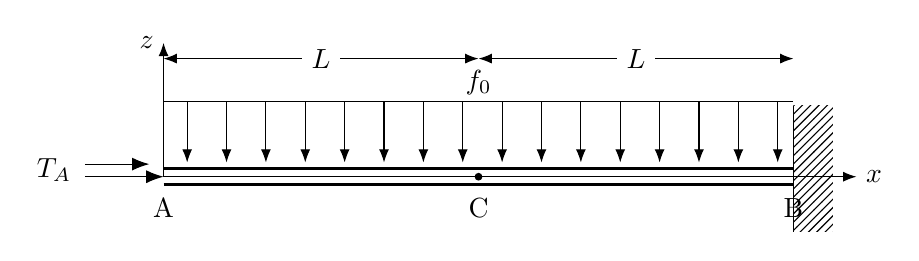
\begin{tikzpicture}[>=Latex]
  \fill[pattern=north east lines] (8,-0.7) rectangle (8.5,0.9);
  \draw (8,-0.7) -- (8,0.9);
  \draw[line width=1.2pt] (0,0.1) -- (8,0.1);
  \draw[line width=1.2pt] (0,-0.1) -- (8,-0.1);
  \draw (0,0.95) -- (8,0.95);
  \foreach \x in {0.3,0.8,...,7.8} {\draw[->] (\x,0.95) -- (\x,0.18);}
  \node at (4.0,1.2) {$f_0$};
  \draw[-{Latex[length=2.2mm]}] (-1.0,0.0) -- (0.0,0.0);
  \draw[-{Latex[length=2.2mm]}] (-1.0,0.16) -- (-0.18,0.16);
  \node[left] at (-1.05,0.08) {$T_A$};
  \draw[->] (0,0) -- (0,1.7) node[left]{$z$};
  \draw[->] (0,0) -- (8.8,0) node[right]{$x$};
  \node[below] at (0,-0.15) {A}; \node[below] at (4,-0.15) {C}; \node[below] at (8,-0.15) {B};
  \fill (4,0) circle (1.4pt);
  \draw[<->] (0,1.5) -- (4,1.5) node[midway,fill=white]{$L$};
  \draw[<->] (4,1.5) -- (8,1.5) node[midway,fill=white]{$L$};
\end{tikzpicture}

\vspace{1mm}
図2
\end{center}

\subsection*{解答}

\noindent\textbf{(1)}\quad 丸棒全体を自由体とみる．下向き等分布荷重の合力は $f_0\cdot 2L$ で，
全長の中央（固定端 B から距離 $L$）に作用する．固定端 B の支持力 $R_B$（上向き），
支持モーメント $M_B$，支持トルク $T_B$ を未知とする．

\begin{center}
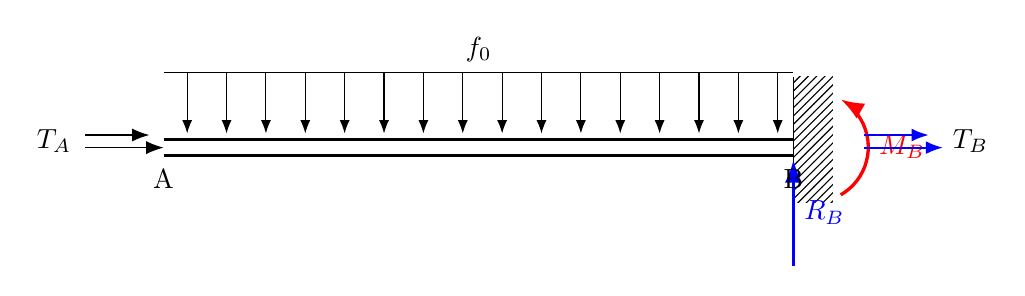
\begin{tikzpicture}[>=Latex]
  \fill[pattern=north east lines] (8,-0.7) rectangle (8.5,0.9);
  \draw (8,-0.7) -- (8,0.9);
  \draw[line width=1.2pt] (0,0.1) -- (8,0.1);
  \draw[line width=1.2pt] (0,-0.1) -- (8,-0.1);
  \draw (0,0.95) -- (8,0.95);
  \foreach \x in {0.3,0.8,...,7.8} {\draw[->] (\x,0.95) -- (\x,0.18);}
  \node at (4.0,1.25) {$f_0$};
  \draw[-{Latex[length=2.2mm]}] (-1.0,0.0) -- (0.0,0.0);
  \draw[-{Latex[length=2.2mm]}] (-1.0,0.16) -- (-0.18,0.16);
  \node[left] at (-1.05,0.08) {$T_A$};
  % 反力
  \draw[->,very thick,blue] (8,-1.5) -- (8,-0.15) node[midway,right]{$R_B$};
  \draw[->,very thick,red] (8.6,-0.6) arc (-60:60:0.7) node[right,midway]{$M_B$};
  \draw[-{Latex[length=2.2mm]},thick,blue] (8.9,0.0) -- (9.9,0.0);
  \draw[-{Latex[length=2.2mm]},thick,blue] (8.9,0.16) -- (9.72,0.16);
  \node[right] at (9.9,0.08) {$T_B$};
  \node[below] at (0,-0.15) {A}; \node[below] at (8,-0.15) {B};
\end{tikzpicture}
\end{center}

鉛直方向のつり合い，および点 B まわりの曲げモーメントのつり合い，軸まわりのねじりのつり合いより
\[
  R_B = \int_0^{2L} f_0\,dx = 2f_0 L,\qquad
  M_B = (f_0\cdot 2L)\cdot L = 2f_0 L^2,\qquad
  T_B = T_A .
\]
\[
  \ans{\;R_B = 2f_0 L\ (\text{上向き}),\quad M_B = 2f_0 L^2,\quad T_B = T_A\;}
\]
検算：鉛直力は $R_B - f_0\cdot 2L = 2f_0L - 2f_0L = 0$ でつり合う ✓．
ねじりトルクは途中に他のトルク負荷がないため，自由端 A の $T_A$ がそのまま B に伝わる．

\medskip
\noindent\textbf{(2)}\quad 自由端 A から $x$ の断面で切り，自由端側（$0\le \xi \le x$）の部分を考える．
この部分に働くのは長さ $x$ の等分布荷重 $f_0$ のみで，合力 $f_0 x$ が断面から $x/2$ の位置にある．
よって曲げモーメントは
\[
  M(x) = \int_0^x f_0 (x-\xi)\,d\xi = \frac{f_0 x^2}{2}.
\]
ねじりトルクは自由端 A の $T_A$ が断面まで一定に伝わるので $T(x)=T_A$．
\[
  \ans{\;M(x) = \frac{f_0 x^2}{2},\qquad T(x) = T_A \qquad (0\le x \le 2L)\;}
\]
検算：固定端 $x=2L$ で $M(2L)=\dfrac{f_0(2L)^2}{2}=2f_0L^2=M_B$ となり (1) と一致 ✓．

\medskip
\noindent\textbf{(3)}\quad 点 C は $x=L$ なので $M_C=\dfrac{f_0 L^2}{2}$，$T_C=T_A$．
丸棒の断面係数を用い，上面（$z=+d/2$）の曲げ垂直応力は引張りとなり
\[
  \sigma_x = \frac{M_C\,(d/2)}{I} = \frac{\dfrac{f_0 L^2}{2}\cdot \dfrac{d}{2}}{\dfrac{\pi d^4}{64}}
           = \frac{16 f_0 L^2}{\pi d^3}.
\]
軸直交方向には荷重がないので $\sigma_y = 0$．ねじりによる表面せん断応力は
\[
  \tau_{xy} = \frac{T_A\,(d/2)}{J} = \frac{T_A \cdot \dfrac{d}{2}}{\dfrac{\pi d^4}{32}}
            = \frac{16 T_A}{\pi d^3}.
\]
\[
  \ans{\;\sigma_x = \frac{16 f_0 L^2}{\pi d^3}\ (\text{引張り}),\quad
        \sigma_y = 0,\quad
        \tau_{xy} = \frac{16 T_A}{\pi d^3}\;}
\]
検算：$\sigma_x$ は $M c/I$，$\tau_{xy}$ は $T r/J$ の標準式に一致．
$I=\dfrac{\pi d^4}{64}$，$J=2I=\dfrac{\pi d^4}{32}$ も整合 ✓．

\medskip
\noindent\textbf{(4)}\quad たわみの基礎式 $EI\,v''=M(x)=\dfrac{f_0 x^2}{2}$ を $x$（A 原点）で2回積分する．
\[
  EI\,v' = \frac{f_0 x^3}{6} + C_1,\qquad
  EI\,v  = \frac{f_0 x^4}{24} + C_1 x + C_2 .
\]
固定端 $x=2L$ での境界条件 $v(2L)=0,\ v'(2L)=0$ より
\[
  C_1 = -\frac{f_0 (2L)^3}{6} = -\frac{4f_0 L^3}{3},\qquad
  C_2 = -\frac{f_0(2L)^4}{24} - C_1(2L) = -\frac{2f_0L^4}{3}+\frac{8f_0L^4}{3} = 2f_0 L^4 .
\]
自由端 A（$x=0$）のたわみは $EI\,v(0)=C_2=2f_0L^4$ なので
\[
  \ans{\;\delta_A = \frac{2 f_0 L^4}{EI} = \frac{2f_0 L^4}{E\cdot \pi d^4/64} = \frac{128\,f_0 L^4}{\pi E d^4}\;}
\]
ねじれ角は全長 $2L$ にわたりトルク $T_A$ 一定なので
\[
  \ans{\;\phi = \frac{T_A\,(2L)}{G J} = \frac{2T_A L}{G\cdot \pi d^4/32} = \frac{64\,L\,T_A}{\pi G d^4}\;}
\]
検算：等分布荷重を受ける片持ちはり（全長 $\ell=2L$）の自由端たわみの公式
$\delta=\dfrac{f_0 \ell^4}{8EI}=\dfrac{f_0(2L)^4}{8EI}=\dfrac{2f_0L^4}{EI}$ と一致する ✓．

\medskip
\noindent\textbf{(5)}\quad カスチリアーノの定理で自由端 A のたわみを求める．
A に下向きの仮想集中荷重 $Q$ を加えると，A から $x$ の断面の曲げモーメントは
\[
  M(x) = \frac{f_0 x^2}{2} + Q x,\qquad \frac{\partial M}{\partial Q} = x .
\]
ひずみエネルギーは曲げのみ寄与する（A のたわみにねじりは関与しない）から
\[
  \delta_A = \left.\frac{\partial U}{\partial Q}\right|_{Q=0}
           = \int_0^{2L} \frac{M}{EI}\frac{\partial M}{\partial Q}\,dx \Bigg|_{Q=0}
           = \frac{1}{EI}\int_0^{2L} \frac{f_0 x^2}{2}\cdot x\,dx .
\]
積分を実行して
\[
  \delta_A = \frac{f_0}{2EI}\int_0^{2L} x^3\,dx
           = \frac{f_0}{2EI}\cdot\frac{(2L)^4}{4}
           = \frac{f_0}{2EI}\cdot 4L^4
           = \frac{2 f_0 L^4}{EI}.
\]
\[
  \ans{\;\delta_A = \frac{2 f_0 L^4}{EI}\quad(\text{下向き})\;}
\]
検算：(4) で基礎式から得た $\delta_A=\dfrac{2f_0L^4}{EI}$ と完全に一致する ✓．

\end{document}
